%------------------------------------------------------------
% DEFINITIONS AND HEADERS -- IGNORE THIS
%------------------------------------------------------------
\documentclass{article}
\usepackage[top=2.25cm, bottom=3cm, left=2.5cm, right=2.4cm]{geometry}
\usepackage[utf8]{inputenc}
\usepackage{algpseudocode}
\usepackage{booktabs}
% Get better typography
\usepackage[protrusion=true,expansion=true]{microtype}  
% For algorithms
\usepackage[boxruled,linesnumbered,vlined,inoutnumbered]{algorithm2e}
\SetKwInOut{Parameter}{Parameters}
% For basic math, align, fonts, etc.
\usepackage{amsmath}
\usepackage{amsthm}
\usepackage{amssymb}
\usepackage{float}
\usepackage{mathtools}
\usepackage{mathrsfs}
\usepackage{rotating}
\usepackage{tabularx}
\usepackage{booktabs}
\usepackage{soul}
\usepackage{changepage}
\usepackage{gensymb} % For \degree
\usepackage{lscape}
% For \thead to make line breaks in tables
\usepackage{array}
\usepackage{makecell}
\renewcommand\theadalign{bc}
\renewcommand\theadfont{\bfseries}
\renewcommand\theadgape{\Gape[4pt]}
\renewcommand\cellgape{\Gape[4pt]}
\usepackage{courier} % For \texttt{foo} to put foo in Courier (for code / variables)
\usepackage{lipsum} % For dummy text
% For images
\usepackage{graphicx}
\usepackage{subcaption}
\usepackage[space]{grffile} % For spaces in image names
% For bibliography
\usepackage[round]{natbib}
% For color
\usepackage{xcolor}
\definecolor{light-grey}{rgb}{0.9,0.9,0.9}
\definecolor{dark-red}{rgb}{0.4,0.15,0.15}
\definecolor{dark-blue}{rgb}{0,0,0.7}
\definecolor{darkblue}{rgb}{0,0,.6}
\definecolor{darkred}{rgb}{.58,0,0}
\definecolor{brighterred}{rgb}{.745,0,0}
\definecolor{darkgreen}{rgb}{0,.6,0}
\definecolor{red}{rgb}{.98,0,0}
\usepackage{environ}
% Only show sections in table of contents and rename
\setcounter{tocdepth}{2}
\renewcommand{\contentsname}{Table of Contents}
% For links (e.g., clicking a reference takes you to the phy)
\usepackage{hyperref}
\hypersetup{
    colorlinks, linkcolor={dark-blue},
    citecolor={dark-blue}, urlcolor={dark-blue}
}
\newcommand{\HIGHLIGHT}[1]{\textcolor{blue}{\textbf{#1}}}
% \newcommand{\Solution}[1]{{\color{blue} \paragraph{\bf $\bigstar $ SOLUTION:} { \sf
%     #1} \bigskip}}
\newcommand{\TODO}[1]{\textcolor{blue}{\textbf{{#1}}}}
\newcommand{\POINTS}[1]{\textcolor{purple}{\textbf{{#1}}}}
\providecommand{\mathcolor}[2]{\textcolor{#1}{#2}}
% My definition of "summary boxes" (see below)
\usepackage[most]{tcolorbox}
\definecolor{boxgray}{rgb}{0.95, 0.95, 0.95}
\definecolor{boxblue}{rgb}{0.941, 0.941, 0.98}
\definecolor{boxpink}{rgb}{1.0, 0.93, 0.93}
\definecolor{boxwhite}{rgb}{1.0, 1.0, 1.0}
%\definecolor{boxgreen}{rgb}{0.91, 0.96, 0.9}
\definecolor{boxgreen}{rgb}{0.92, 0.96, 0.92}
\newtcolorbox{mybox}[1][boxwhite]{%
  enhanced,
  boxrule=0.5pt,
  colframe=black,
  colback=#1,
  sharp corners,
  width=\linewidth,
  left=1em,
  right=1em,
  top=0.5em,
  bottom=0.5em,
  boxsep=0pt,
  before skip=1em,
  after skip=0.85em,
}
%------------------------------------------------------------




\begin{document}
%-----------------
%   Homework 3
%-----------------
\newpage
\vspace*{1cm}
\begin{center}
    \begin{Large}
    COMPSCI 589 Homework 3 - Spring 2026
    \end{Large}
    \\
    \vspace{0.15cm}
    Due \textcolor{darkred}{\textbf{March 30}}, 11:55 pm Eastern Time
\end{center}
\addcontentsline{toc}{subsection}{\textbf{Homework 3}}




%---- Instructions ----------------------

\vspace{0.5cm}
\section*{Instructions}
\vspace{0.5cm}

\begin{itemize}
    \item This homework assignment consists of a programming part. 
    \item While you may discuss problems with your peers (e.g., to discuss high-level approaches), you must answer the questions on your own and implement all solutions independently. In your submission, do explicitly list all students with whom you discussed this assignment. 
    \item Submissions must be typed. You must use \LaTeX to prepare your submission. Handwritten and scanned submissions will not be accepted. 
    \item The written report, including your answers, plots, and analysis, should be submitted on Gradescope as a PDF via the appropriate submission link. The source code should be submitted as a single .zip file through the separate programming assignment link on Gradescope.
    \item We strongly encourage using Python 3 for your homework code. You may use other languages. In either case, you \textit{must} provide clear instructions for running your code and reproducing your experiments. 
    \item You \textit{may not} use any machine learning-specific libraries in your code, e.g., TensorFlow, PyTorch, or machine learning algorithms implemented in scikit-learn (though you \textit{may} use other functions provided by this library, such as one that splits a dataset into training and testing sets). You may also use libraries such as numpy and matplotlib. If you are not certain whether a specific library is allowed, do ask us.
    \item All submissions will be checked for plagiarism using two independent plagiarism-detection tools. Renaming variable or function names, moving code within a file, etc., are all strategies that \textit{do not} fool the plagiarism-detection tools we use. Your code will also be compared with submissions from your classmates and with publicly available implementations online. 
    \item \textcolor{red}{If you get caught, all penalties mentioned in the syllabus \textit{will} be applied---which may include directly failing the course with a letter grade of ``F''}.
    \begin{center}
        \textcolor{red}{$\rightarrow$ Before starting this homework, please review this course's policies on plagiarism by  \\reading the corresponding section of the syllabus.}
    \end{center}
    \item The automated system will not accept assignments after 11:55 pm on March 30. 
    \item The TeX file for this homework (which you should use to write your solutions in \LaTeX), as well as the datasets you will investigate, are available on Canvas under ``\textit{Homework \#3 - Supporting Files}''. See below for more details.
\end{itemize}

% --------------------






%------ High-Level Overview of the Homework --------------------------
\newpage
\noindent {\LARGE{\textbf{Programming Assignment}} \POINTS{[100 Points, total]}}
\vspace{0.5cm}

\noindent In this homework, you will be implementing the Random Forest algorithm. \textbf{Notice that you may \ul{not} use existing machine learning code for this problem: you must implement the learning algorithms entirely on your own and from scratch.} 
\vspace{0.5cm}

\noindent In this assignment, you will:

\begin{itemize}
\item Leverage your implementation of the standard Decision Tree algorithm, based on the Information Gain splitting criterion, to implement a Random Forest classifier.
%
\begin{mybox}[boxpink] 
\textbf{Important}:
You must reuse \textbf{\textcolor{darkred}{\textit{your}}} previous implementation of the Decision Tree algorithm.
\end{mybox}
%
\begin{mybox}[boxblue] 
\textbf{Important}:
Your implementation of the Decision Tree algorithm should support both categorical \textbf{\textcolor{darkred}{\textit{and}}} numerical attributes. When determining the numerical threshold to use when splitting numerical nodes, you may \textit{(i)} use the average of that attribute's values in the partition of instances associated with the current node; or \textit{(ii)} use the more sophisticated (and ``powerful'') technique discussed in Lecture 05. 
\end{mybox}
%
\item Implement a procedure to create bootstrap datasets by sampling (\textit{with replacement}) from the current training set to construct the datasets based on which each tree in the random forest will be trained. 
\item Implement a mechanism to select (whenever a node is being split) $m$ attributes at random from the complete set of attributes of an instance. You should then split the node based on the attribute with the best Information Gain. As a heuristic, we usually use $m \approx \sqrt{X}$, where $X$ is the total number of attributes in each instance of the dataset.
\item Implement a majority voting mechanism that takes into account the predictions made by each tree in the ensemble to classify new instances.
\item Implement the \textit{stratified cross-validation} technique to evaluate the generalization capability of the random forest. For an example of how this technique works, see Figure~\ref{fig:cross-val}. We recommend using $k=5$ folds. Of these, $k-1$ folds will be used to train a random forest composed of $ntree$ trees. Here, \textbf{$ntree$ will be the main adjustable hyperparameter of your algorithm}. 
%
\begin{mybox}[boxpink] 
\textbf{Note}:
In cross-validation, the remaining fold (the one not used during training) will be used to evaluate the performance of the random forest itself (\textcolor{darkred}{i.e., \underline{not} the performance of any individual tree separately!}). 
\end{mybox}
%
Another way to describe how cross-validation works in our setting is as follows: at each iteration of the cross-validation process, you will train not only \textit{one} decision tree, but multiple ($ntree$) decision trees, all of which will be combined to form your random forest. You will then repeat this process, training and evaluating $k$ random forests (one for each of the $k$ cross-validation iterations). The final cross-validation performance you should return is the average of the performances computed for each of the folds.
\item Evaluate the impact the number of trees (i.e., the $ntree$ hyperparameter) has on the performance of your random forest.
%
\end{itemize}


\newpage
\vspace{2cm}

    \begin{figure}[ht!!]
        \centering
        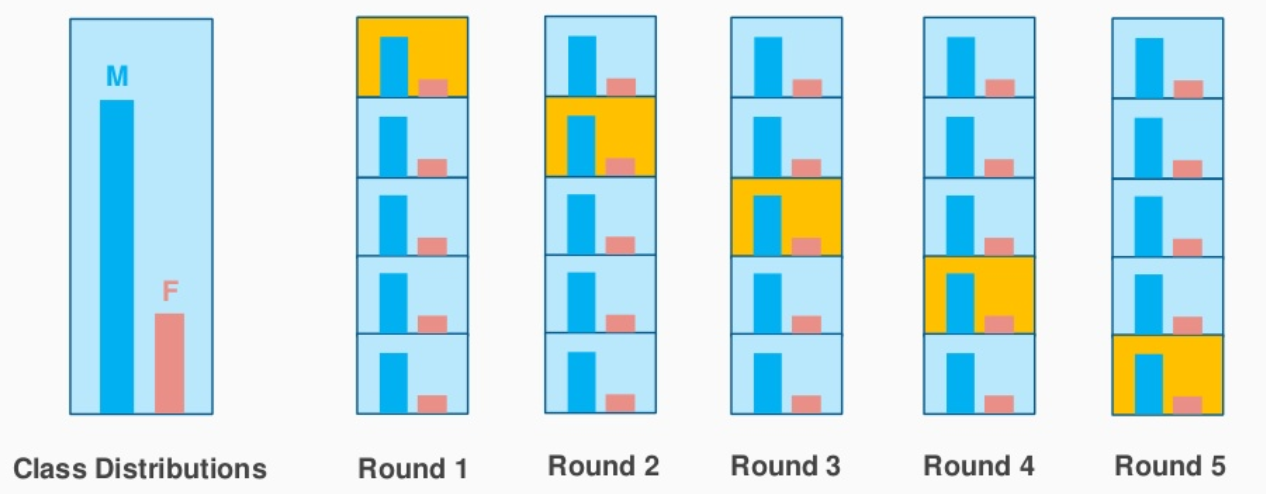
\includegraphics[width=0.75\textwidth]{figures/HW3_cross_val_stratified2.png}
        \caption{Example of how to construct \textit{stratified} folds to perform $k$-fold cross-validation. Here, we assume two classes: \textbf{\texttt{M}} and \textbf{\texttt{F}}. Notice how the complete dataset (shown in the leftmost figure) is not balanced: approximately 3/4 of its instances belong to the class \textbf{\texttt{M}}, and approximately $1/4$ of its instances belong to the class \textbf{\texttt{F}}. We wish to approximately preserve these proportions (i.e., the proportion of instances of class \textbf{\texttt{M}} and the proportion of instances of class \textbf{\texttt{F}}) in each of the $k=5$ folds. To do this, you should first split the original dataset, $D$, into two: one containing only instances of class \textbf{\texttt{M}} (sub-dataset $D_M$), and another one containing only instances of class  \textbf{\texttt{F}} (sub-dataset $D_F$). Then, given the total number of instances in the original dataset ($D$) and the number of folds you are using ($k$), you should be able to determine the size of each fold. Let us assume that each fold, in this example, should have $50$ instances. To construct each fold, you should draw random instances from $D_M$ and $D_F$. In this example, $3/4$ of the instances that you add to the current fold should come from $D_M$, and $1/4$ of the instances that you add to the current fold should come from $D_F$. Notice that because the folds should be disjoint (i.e., an instance should appear in only one fold), after drawing an instance either from $D_M$ or $D_F$, it should be removed from such a set to ensure that it will not be accidentally included as part of another fold. \textit{(Source: \href{https://stats.stackexchange.com/questions/49540/understanding-stratified-cross-validation}{Stack Exchange})}.}
        \label{fig:cross-val}
    \end{figure}



\newpage

%------ Description of the Expected Deliverables --------------------------
\section{Deliverables and Datasets}

The main objective of this homework is to study the impact of the number of trees in a random forest (i.e., the $ntree$ hyperparameter) on its performance. \textbf{When constructing each tree in the ensemble, you are free to choose among several stopping criteria}. You may, for instance:


\begin{itemize} 
\item Stop splitting nodes whenever the data partition associated with the current node contains fewer than $n$ instances, for some value of $n$ that you choose empirically. We will refer to this as the \texttt{minimum\_size\_for\_split} criterion.
\item Stop splitting nodes whenever the information gain resulting from a split is not sufficiently high (even if it is slightly greater than zero). You are free to choose empirically the minimum information gain you would like to use. We will refer to this as the \texttt{minimum\_gain} criterion.
\item You may stop splitting whenever the current branch of the tree becomes too deep, that is, when its depth exceeds some pre-defined value that you select empirically. We will refer to this as the \texttt{maximum\_depth} stopping criterion.
\end{itemize}
%
\begin{mybox}[boxpink] 
\textbf{Important:} In all questions below, you should explicitly mention which criterion or criteria you used and the corresponding hyperparameter(s). You should try different options to identify the setting that produces the best possible performance for your algorithm.
\end{mybox}
%





%------ Description of the Datasets --------------------------
\noindent In this homework, you will be analyzing two datasets:
\vspace{0.3cm}

\noindent \textbf{(1) \textcolor{darkblue}{\ul{The Wisconsin Breast Cancer Diagnostic (WDBC) Dataset}}.}
\noindent The goal here is to train a classifier capable of predicting whether a breast mass is malignant or benign, based on features computed from a digitized image of a breast mass. The dataset is composed of 569 instances. Each instance is described by 30 \textit{numerical} attributes, and there are two classes.
\vspace{0.5cm}

\noindent \textbf{(2) \textcolor{darkblue}{\ul{The Loan Eligibility Prediction Dataset}}.}
\noindent Here, the goal is to automatically (and accurately) predict whether a given person should qualify for a loan. Each instance is described by 11 attributes, including the gender of the applicant, whether the applicant is married, their income, information about their credit history, etc. The binary target class to be predicted is whether a given applicant's request for a loan was approved or not. Notice that this dataset contains 7 \textit{categorical} attributes and 4 \textit{numerical} attributes. There is a total of 480 instances in the dataset. 
\vspace{0.3cm}

\begin{mybox}[boxblue] 
\textbf{Note:} The datasets above can be found in the ``\textit{Supporting Files}'' zip file for this homework on Canvas.
\end{mybox}




\newpage


%------ Main Questions --------------------------
\vspace{0.7cm}
\section{Questions}

For each dataset, you should:

\begin{enumerate}
    \item Train a random forest and evaluate it using the stratified cross-validation technique discussed above. You should train random forests with different values of the $ntree$ parameter: 1, 5, 10, 20, 30, 40, and 50.

    \item For each value of $ntree$, you should measure the accuracy, precision, recall, and F1 score of the resulting random forest. 

\noindent \textbf{WDBC} Hyperparameter ($k=5$, \textt{max\_depth}=8, \texttt{min\_samples\_split}=2)

\noindent \textbf{Loan} Hyperparameter ($k=5$, \textt{max\_depth}=5, \texttt{min\_samples\_split}=2)
    
\begin{table}[htbp]
\centering
\caption{WDBC Result ($k=5$, \texttt{max\_depth}=8, \texttt{min\_samples\_split}=2)}
\label{tab:wdbc_result}
\begin{tabular}{ccccc}
\toprule
ntrees & acc & prec & recall & f1 \\
\midrule
1  & 0.913921 & 0.928642 & 0.935563 & 0.931813 \\
5  & 0.941993 & 0.942741 & 0.966354 & 0.954341 \\
10 & 0.950720 & 0.953431 & 0.969131 & 0.961043 \\
20 & 0.957768 & 0.957035 & 0.977543 & 0.966867 \\
30 & 0.971835 & 0.970122 & 0.985955 & 0.977832 \\
40 & 0.968357 & 0.964898 & 0.985955 & 0.975148 \\
50 & 0.964848 & 0.959446 & 0.985955 & 0.972408 \\
\bottomrule
\end{tabular}
\end{table}

\begin{table}[htbp]
\centering
\caption{Loan Result ($k=5$, \texttt{max\_depth}=5, \texttt{min\_samples\_split}=2)}
\label{tab:loan_result}
\begin{tabular}{ccccc}
\toprule
ntrees & acc & prec & recall & f1 \\
\midrule
1  & 0.731248 & 0.773090 & 0.867662 & 0.816866 \\
5  & 0.803956 & 0.791307 & 0.975893 & 0.873558 \\
10 & 0.804021 & 0.793959 & 0.969878 & 0.872832 \\
20 & 0.797770 & 0.791954 & 0.963953 & 0.868734 \\
30 & 0.801850 & 0.791301 & 0.972908 & 0.872178 \\
40 & 0.801894 & 0.792679 & 0.969923 & 0.871776 \\
50 & 0.803956 & 0.793142 & 0.972908 & 0.873284 \\
\bottomrule
\end{tabular}
\end{table}

\newpage
    \item You should then create, for each dataset and for each of the four metrics described above, a graph that shows the value of $ntree$ on the x-axis and the value of the corresponding metric on the y-axis. For example, you should include one graph showing the accuracy of the random forest as a function of $ntree$ for \texttt{Dataset \#1}, another graph showing the precision of the random forest as a function of $ntree$ for \texttt{Dataset \#1}, and similar graphs for the other metrics and for \texttt{Dataset \#2}.
    %
    \begin{mybox}[boxpink] 
    \textbf{Important:} The analyses mentioned above should result in a total of \textcolor{darkred}{\ul{\textbf{8 graphs}}}. Please indicate clearly in the caption of each figure/graph which results are shown in that graph.
    \end{mybox}
    %

\noindent \textbf{WDBC} Hyperparameter ($k=5$, \textt{max\_depth}=8, \texttt{min\_samples\_split}=2)

\noindent \textbf{Loan} Hyperparameter ($k=5$, \textt{max\_depth}=5, \texttt{min\_samples\_split}=2)

\noindent \textbf{WDBC:}
\begin{figure}[H]
    \centering
    \begin{minipage}[t]{0.48\textwidth}
        \centering
        
\includegraphics[width=\textwidth]{/home/zichenw/Downloads/cs589_HW/HW3/HW3_CMPSCI_589_Spring2026_Supporting_Files/latex_source/wdbc_k5_depth8_minsplit2/WDBC_5_depth_8_minsplit2_acc.png}
        \caption{Accuracy for WDBC dataset.}
        \label{fig:wdbc-acc}
    \end{minipage}
    \hfill
    \begin{minipage}[t]{0.48\textwidth}
        \centering
        
\includegraphics[width=\textwidth]{/home/zichenw/Downloads/cs589_HW/HW3/HW3_CMPSCI_589_Spring2026_Supporting_Files/latex_source/wdbc_k5_depth8_minsplit2/WDBC_5_depth_8_minsplit2_recall.png}
        \caption{Recall for WDBC dataset.}
        \label{fig:wdbc-recall}
    \end{minipage}
\end{figure}


\begin{figure}[H]
    \centering
    \begin{minipage}[t]{0.48\textwidth}
        \centering
        
\includegraphics[width=\textwidth]{/home/zichenw/Downloads/cs589_HW/HW3/HW3_CMPSCI_589_Spring2026_Supporting_Files/latex_source/wdbc_k5_depth8_minsplit2/WDBC_5_depth_8_minsplit2_prec.png}
        \caption{Precision for WDBC dataset.}
        \label{fig:wdbc-acc}
    \end{minipage}
    \hfill
    \begin{minipage}[t]{0.48\textwidth}
        \centering
        
\includegraphics[width=\textwidth]{/home/zichenw/Downloads/cs589_HW/HW3/HW3_CMPSCI_589_Spring2026_Supporting_Files/latex_source/wdbc_k5_depth8_minsplit2/WDBC_5_depth_8_minsplit2_f1.png}
        \caption{F1 for WDBC dataset.}
        \label{fig:wdbc-recall}
    \end{minipage}
\end{figure}

\newpage

\noindent \textbf{Loan:}
\begin{figure}[H]
    \centering
    \begin{minipage}[t]{0.48\textwidth}
        \centering
        
\includegraphics[width=\textwidth]{/home/zichenw/Downloads/cs589_HW/HW3/HW3_CMPSCI_589_Spring2026_Supporting_Files/latex_source/loan_k5_depth5_minsplit2/Loan_5_depth_5_minsplit2_acc.png}
        \caption{Accuracy for Loan dataset.}
        \label{fig:wdbc-acc}
    \end{minipage}
    \hfill
    \begin{minipage}[t]{0.48\textwidth}
        \centering
        
\includegraphics[width=\textwidth]{/home/zichenw/Downloads/cs589_HW/HW3/HW3_CMPSCI_589_Spring2026_Supporting_Files/latex_source/loan_k5_depth5_minsplit2/Loan_5_depth_5_minsplit2_recall.png}
        \caption{Recall for Loan dataset.}
        \label{fig:wdbc-recall}
    \end{minipage}
\end{figure}


\begin{figure}[H]
    \centering
    \begin{minipage}[t]{0.48\textwidth}
        \centering

\includegraphics[width=\textwidth]{/home/zichenw/Downloads/cs589_HW/HW3/HW3_CMPSCI_589_Spring2026_Supporting_Files/latex_source/loan_k5_depth5_minsplit2/Loan_5_depth_5_minsplit2_prec.png}
        \caption{Precision for Loan dataset.}
        \label{fig:wdbc-acc}
    \end{minipage}
    \hfill
    \begin{minipage}[t]{0.48\textwidth}
        \centering
        
\includegraphics[width=\textwidth]{/home/zichenw/Downloads/cs589_HW/HW3/HW3_CMPSCI_589_Spring2026_Supporting_Files/latex_source/loan_k5_depth5_minsplit2/Loan_5_depth_5_minsplit2_f1.png}
        \caption{F1 for Loan dataset.}
        \label{fig:wdbc-recall}
    \end{minipage}
\end{figure}

\newpage

    \item For each metric being evaluated (and for each dataset), discuss which value of $ntree$ you would select if you were to deploy this classifier in real life. Explain your reasoning. 

\noindent \textbf{WDBC} Hyperparameter ($k=5$, \textt{max\_depth}=8, \texttt{min\_samples\_split}=2)

\noindent \textbf{Loan} Hyperparameter ($k=5$, \textt{max\_depth}=5, \texttt{min\_samples\_split}=2)



\textbf{WDBC ntree:}
\begin{itemize}
    \item Accuracy: 30\\
because it gives the highest accuracy.
    \item Precision: 30\\
because it gives the highest precision.
    \item Recall: 30/40/50\\
because these three values achieve the same highest recall.
    \item F1: 30\\
because it gives the highest f1.
\end{itemize}

\textbf{Loan ntree:}
\begin{itemize}
    \item Accuracy: 10\\
because it gives the highest accuracy.
    \item Precision: 10\\
because it gives the highest precision.
    \item Recall: 5\\
because it gives the highest recall.
    \item F1: 5\\
because it gives the highest f1.
\end{itemize}


\newpage
    \item Discuss, at a high level, which metrics were more directly affected by changes in the value of $ntree$ and, more generally, how these changes influenced the performance of your algorithm. For example, was the accuracy of the random forest particularly sensitive to increasing $ntree$ beyond a certain value? Was the F1 score a ``harder'' metric to optimize, possibly requiring a larger number of trees in the ensemble? Is there a point beyond which adding more trees does not improve performance (or even makes it worse)?\\

For WDBC, all four metrics increase as ntree increases, showing a monotonic rise from 1 to 30: accuracy improves from 0.913921 to 0.971835, precision from 0.928642 to 0.970122, recall from 0.935563 to 0.985955, and F1 from 0.931813 to 0.977832. However, when ntree was further increased from 30 to 40 and 50, accuracy, precision, and F1 all decreased slightly, while recall remained at its peak value. On the WDBC dataset, accuracy, precision, and F1 are more sensitive to changes in ntree, whereas recall quickly reaches a plateau after reaching a high level. The optimal ntree hyperparameter for WDBC is 30; values above this do not yield further gains and may even result in a slight decline.\\

Loan improved significantly as ntree increased from 1 to 5, but after that, most metrics fluctuated only within a narrow range. Accuracy fluctuated between 0.797770 and 0.804021; precision fluctuated between 0.791 and 0.794; F1 fluctuates between 0.869 and 0.874. Recall remains consistently high, fluctuating around 0.975893. For Loan, accuracy, F1, precision, and recall are all insensitive to ntree. Increasing the value of ntree does not significantly improve these metrics and the optimal value for the ntree hyperparameter is 5.

\end{enumerate}





%-------- Extra Credit Questions --------------------------
\newpage
% \vspace{0.5in}
% \noindent\rule{\textwidth}{1pt}
% \vspace{0.08cm}
\noindent \textcolor{purple}{\textbf{\Large{Extra Credit Questions}}}
\vspace{0.8cm}

\noindent There are two ways in which you may receive extra credit in this homework.
\vspace{0.75cm}



    %---- Extra Credit Question QE.1 ----------------------
    \noindent \textbf{\HIGHLIGHT{[QE.1] Extra points~(\POINTS{10 Points})}} Analyze a third dataset: the \textcolor{darkred}{\textbf{\ul{Raisins Dataset}}}. The goal here is to use morphological features extracted from raisin images to classify each instance as either a Kecimen or a Besni raisin variety. The dataset contains 900 instances. Each instance is described by 7 \textit{numerical} features, and the dataset contains two classes. You should present the same analyses and graphs discussed above.
    %
    \begin{mybox}[boxgray] 
    This dataset can be found in the ``\textit{Supporting Files}'' zip file for this homework on Canvas.
    \end{mybox}


\section*{Questions}

For each dataset, you should:

\begin{enumerate}
    \item Train a random forest and evaluate it using the stratified cross-validation technique discussed above. You should train random forests with different values of the $ntree$ parameter: 1, 5, 10, 20, 30, 40, and 50.

    \item For each value of $ntree$, you should measure the accuracy, precision, recall, and F1 score of the resulting random forest. 

\noindent \textbf{Raisin} Hyperparameter ($k=5$, \textt{max\_depth}=10, \texttt{min\_samples\_split}=5)

\begin{table}[htbp]
\centering
\caption{Raisin Result ($k=5$, \texttt{max\_depth}=10, \texttt{min\_samples\_split}=5)}
\label{tab:raisin_result}
\begin{tabular}{ccccc}
\toprule
ntrees & acc & prec & recall & f1 \\
\midrule
1  & 0.796667 & 0.805997 & 0.784444 & 0.793242 \\
5  & 0.832222 & 0.849506 & 0.808889 & 0.828039 \\
10 & 0.855556 & 0.889168 & 0.813333 & 0.848870 \\
20 & 0.856667 & 0.885104 & 0.820000 & 0.851053 \\
30 & 0.868889 & 0.897423 & 0.833333 & 0.863826 \\
40 & 0.864444 & 0.894308 & 0.826667 & 0.858862 \\
50 & 0.863333 & 0.896393 & 0.822222 & 0.857330 \\
\bottomrule
\end{tabular}
\end{table}


\newpage
    \item You should then create, for each dataset and for each of the four metrics described above, a graph that shows the value of $ntree$ on the x-axis and the value of the corresponding metric on the y-axis. For example, you should include one graph showing the accuracy of the random forest as a function of $ntree$ for \texttt{Dataset \#1}, another graph showing the precision of the random forest as a function of $ntree$ for \texttt{Dataset \#1}, and similar graphs for the other metrics and for \texttt{Dataset \#2}.
    %
    \begin{mybox}[boxpink] 
    \textbf{Important:} The analyses mentioned above should result in a total of \textcolor{darkred}{\ul{\textbf{8 graphs}}}. Please indicate clearly in the caption of each figure/graph which results are shown in that graph.
    \end{mybox}
    %

\noindent \textbf{Raisin} Hyperparameter ($k=5$, \textt{max\_depth}=10, \texttt{min\_samples\_split}=5)

\noindent \textbf{Raisin:}
\begin{figure}[H]
    \centering
    \begin{minipage}[t]{0.48\textwidth}
        \centering
        
\includegraphics[width=\textwidth]{/home/zichenw/Downloads/cs589_HW/HW3/HW3_CMPSCI_589_Spring2026_Supporting_Files/latex_source/raisin_k5_depth10_minsplit5/Raisin_5_depth_10_minsplit5_acc.png}
        \caption{Accuracy for Raisin dataset.}
        \label{fig:raisin-acc}
    \end{minipage}
    \hfill
    \begin{minipage}[t]{0.48\textwidth}
        \centering
        
\includegraphics[width=\textwidth]{/home/zichenw/Downloads/cs589_HW/HW3/HW3_CMPSCI_589_Spring2026_Supporting_Files/latex_source/raisin_k5_depth10_minsplit5/Raisin_5_depth_10_minsplit5_recall.png}
        \caption{Recall for Raisin dataset.}
        \label{fig:raisin-recall}
    \end{minipage}
\end{figure}


\begin{figure}[H]
    \centering
    \begin{minipage}[t]{0.48\textwidth}
        \centering

\includegraphics[width=\textwidth]{/home/zichenw/Downloads/cs589_HW/HW3/HW3_CMPSCI_589_Spring2026_Supporting_Files/latex_source/raisin_k5_depth10_minsplit5/Raisin_5_depth_10_minsplit5_prec.png}
        \caption{Precision for Raisin dataset.}
        \label{fig:raisin-acc}
    \end{minipage}
    \hfill
    \begin{minipage}[t]{0.48\textwidth}
        \centering
        
\includegraphics[width=\textwidth]{/home/zichenw/Downloads/cs589_HW/HW3/HW3_CMPSCI_589_Spring2026_Supporting_Files/latex_source/raisin_k5_depth10_minsplit5/Raisin_5_depth_10_minsplit5_f1.png}
        \caption{F1 for Raisin dataset.}
        \label{fig:raisin-recall}
    \end{minipage}
\end{figure}

\newpage

    \item For each metric being evaluated (and for each dataset), discuss which value of $ntree$ you would select if you were to deploy this classifier in real life. Explain your reasoning. 

\noindent \textbf{Raisin} Hyperparameter ($k=5$, \textt{max\_depth}=10, \texttt{min\_samples\_split}=5)

\textbf{Raisin ntree:}
\begin{itemize}
    \item Accuracy: 30\\
because it gives the highest accuracy.
    \item Precision: 30\\
because it gives the highest precision.
    \item Recall: 30\\
because these three values achieve the same highest recall.
    \item F1: 30\\
because it gives the highest f1.
\end{itemize}

\newpage
    \item Discuss, at a high level, which metrics were more directly affected by changes in the value of $ntree$ and, more generally, how these changes influenced the performance of your algorithm. For example, was the accuracy of the random forest particularly sensitive to increasing $ntree$ beyond a certain value? Was the F1 score a ``harder'' metric to optimize, possibly requiring a larger number of trees in the ensemble? Is there a point beyond which adding more trees does not improve performance (or even makes it worse)?\\

For Raisin, all four metrics increase as ntree increases, showing a monotonic rise from 1 to 30. On the Raisin dataset, accuracy, precision, recall and F1 are more sensitive to changes in ntree. The optimal ntree hyperparameter for WDBC is 30; values above this do not yield further gains and may even result in a slight decline.\\
\end{enumerate}






\newpage
    %---- Extra Credit Question QE.2 ----------------------
    \vspace{1.0cm}
    \noindent \textbf{\HIGHLIGHT{[QE.2] Extra points~(\POINTS{10 Points})}} Analyze a fourth dataset: the \textcolor{darkred}{\textbf{\ul{Titanic Dataset}}}. On April 15, 1912, the largest passenger liner ever made collided with an iceberg during her maiden voyage. When the Titanic sank, it killed 1502 out of 2224 passengers and crew. One of the reasons the shipwreck resulted in such loss of life was that there were not enough lifeboats for the passengers and crew. Although luck was involved in surviving the sinking, some groups of people were more likely to survive than others. The goal here is to predict whether a given person was likely to survive this tragedy. The dataset contains data for 887 real passengers of the Titanic. Each row represents one person. The columns describe different attributes of the person, including whether they survived (the class/label), their age, their passenger class, sex, and the fare they paid. Notice that this dataset combines \textit{both numerical and categorical attributes}. You should present the same analyses and graphs discussed above.
    %
    \begin{mybox}[boxgray] 
    This dataset can be found in the ``\textit{Supporting Files}'' zip file for this homework on Canvas.
    \end{mybox}


\section*{Questions}

For each dataset, you should:

\begin{enumerate}
    \item Train a random forest and evaluate it using the stratified cross-validation technique discussed above. You should train random forests with different values of the $ntree$ parameter: 1, 5, 10, 20, 30, 40, and 50.

    \item For each value of $ntree$, you should measure the accuracy, precision, recall, and F1 score of the resulting random forest. 

\noindent \textbf{Titanic} Hyperparameter ($k=5$, \textt{max\_depth}=15, \texttt{min\_samples\_split}=2)

\begin{table}[htbp]
\centering
\caption{Titanic Result ($k=5$, \texttt{max\_depth}=15, \texttt{min\_samples\_split}=2)}
\label{tab:titanic_result}
\begin{tabular}{ccccc}
\toprule
ntrees & acc & prec & recall & f1 \\
\midrule
1  & 0.758782 & 0.676421 & 0.722208 & 0.697703 \\
5  & 0.817336 & 0.788254 & 0.725064 & 0.754321 \\
10 & 0.817336 & 0.812804 & 0.692924 & 0.746419 \\
20 & 0.821869 & 0.820099 & 0.695993 & 0.751529 \\
30 & 0.815115 & 0.804686 & 0.693180 & 0.743208 \\
40 & 0.818504 & 0.818334 & 0.684399 & 0.744327 \\
50 & 0.817368 & 0.818164 & 0.684356 & 0.743630 \\
\bottomrule
\end{tabular}
\end{table}


\newpage
    \item You should then create, for each dataset and for each of the four metrics described above, a graph that shows the value of $ntree$ on the x-axis and the value of the corresponding metric on the y-axis. For example, you should include one graph showing the accuracy of the random forest as a function of $ntree$ for \texttt{Dataset \#1}, another graph showing the precision of the random forest as a function of $ntree$ for \texttt{Dataset \#1}, and similar graphs for the other metrics and for \texttt{Dataset \#2}.
    %
    \begin{mybox}[boxpink] 
    \textbf{Important:} The analyses mentioned above should result in a total of \textcolor{darkred}{\ul{\textbf{8 graphs}}}. Please indicate clearly in the caption of each figure/graph which results are shown in that graph.
    \end{mybox}
    %

\noindent \textbf{Titanic} Hyperparameter ($k=5$, \textt{max\_depth}=15, \texttt{min\_samples\_split}=2)

\noindent \textbf{Titanic:}
\begin{figure}[H]
    \centering
    \begin{minipage}[t]{0.48\textwidth}
        \centering
        
\includegraphics[width=\textwidth]{/home/zichenw/Downloads/cs589_HW/HW3/HW3_CMPSCI_589_Spring2026_Supporting_Files/latex_source/titanic_k5_depth15_minsplit2/titanic_5_depth_15_minsplit2_acc.png}
        \caption{Accuracy for Titanic dataset.}
        \label{fig:titanic-acc}
    \end{minipage}
    \hfill
    \begin{minipage}[t]{0.48\textwidth}
        \centering
        
\includegraphics[width=\textwidth]{/home/zichenw/Downloads/cs589_HW/HW3/HW3_CMPSCI_589_Spring2026_Supporting_Files/latex_source/titanic_k5_depth15_minsplit2/titanic_5_depth_15_minsplit2_recall.png}
        \caption{Recall for Titanic dataset.}
        \label{fig:titanic-recall}
    \end{minipage}
\end{figure}


\begin{figure}[H]
    \centering
    \begin{minipage}[t]{0.48\textwidth}
        \centering

\includegraphics[width=\textwidth]{/home/zichenw/Downloads/cs589_HW/HW3/HW3_CMPSCI_589_Spring2026_Supporting_Files/latex_source/titanic_k5_depth15_minsplit2/titanic_5_depth_15_minsplit2_prec.png}
        \caption{Precision for Titanic dataset.}
        \label{fig:titanic-acc}
    \end{minipage}
    \hfill
    \begin{minipage}[t]{0.48\textwidth}
        \centering
        
\includegraphics[width=\textwidth]{/home/zichenw/Downloads/cs589_HW/HW3/HW3_CMPSCI_589_Spring2026_Supporting_Files/latex_source/titanic_k5_depth15_minsplit2/titanic_5_depth_15_minsplit2_f1.png}
        \caption{F1 for Titanic dataset.}
        \label{fig:titanic-recall}
    \end{minipage}
\end{figure}

\newpage

    \item For each metric being evaluated (and for each dataset), discuss which value of $ntree$ you would select if you were to deploy this classifier in real life. Explain your reasoning. 

\noindent \textbf{Titanic} Hyperparameter ($k=5$, \textt{max\_depth}=15, \texttt{min\_samples\_split}=2)

\textbf{Titanic ntree:}
\begin{itemize}
    \item Accuracy: 20\\
because it gives the highest accuracy.
    \item Precision: 20\\
because it gives the highest precision.
    \item Recall: 5\\
because these three values achieve the same highest recall.
    \item F1: 5\\
because it gives the highest f1.
\end{itemize}

\newpage
    \item Discuss, at a high level, which metrics were more directly affected by changes in the value of $ntree$ and, more generally, how these changes influenced the performance of your algorithm. For example, was the accuracy of the random forest particularly sensitive to increasing $ntree$ beyond a certain value? Was the F1 score a ``harder'' metric to optimize, possibly requiring a larger number of trees in the ensemble? Is there a point beyond which adding more trees does not improve performance (or even makes it worse)?\\

For Titanic, different metrics respond differently to changes in ntree: accuracy and precision peak at ntree = 20, while recall and F1 score peak at ntree = 5. There is no single ntree value that optimizes all metrics simultaneously on the Titanic dataset. Furthermore, for the Titanic dataset, increasing ntree from 1 to 5 or 20 yields significant improvements; however, after increasing from 20 to 30, 40, or 50, neither accuracy nor F1 score continues to rise slowly, and some metrics even decrease slightly.

\end{enumerate}






\end{document}

